\section{Optimization}

\subsection{Restrictions}
As a reminder: $L$ is the length of the robot, and $w$ the width of the flywheel cylinders.
\begin{enumerate}
\item Not crashing with the ground at any inclination can be translated as:
\begin{figure}[ht]
	\centering
	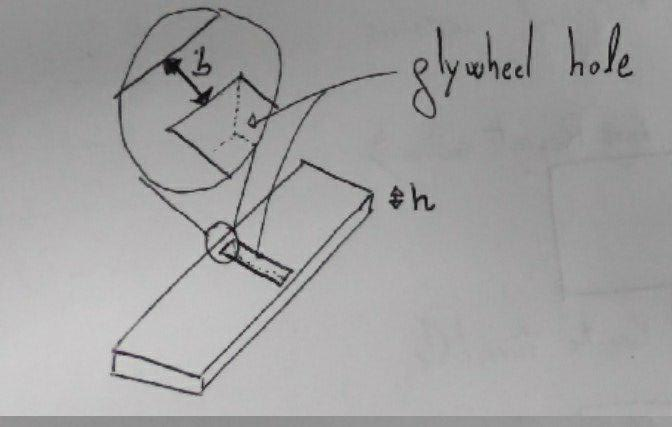
\includegraphics[width=5cm]{img/flywheel_hole.jpg}
	\caption{Flywheel hole diagram}
	\label{fig:Flywheel hole diagram}
\end{figure}
\[r_{wheel}> \sqrt{(r_{flywheel} + b)^2+\frac{h}{2}^2} + 2*\epsilon\]
\item We want to inserted the robot in to a external of diameter 0.5m so:
\begin{figure}[ht]
	\centering
	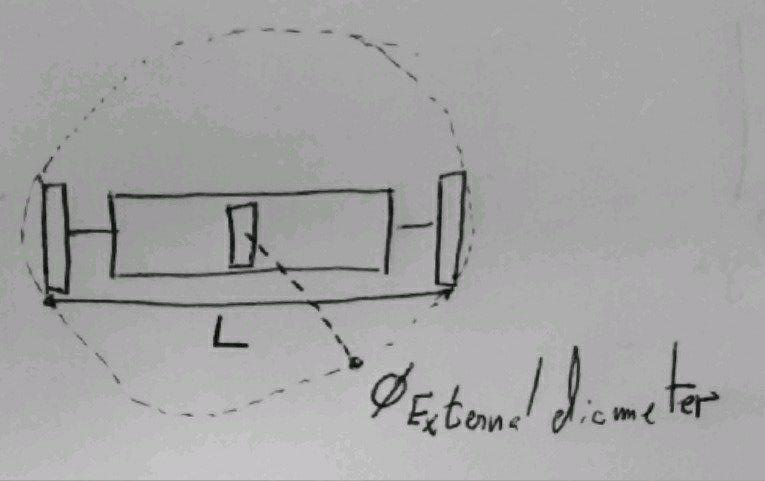
\includegraphics[width=5cm]{img/external_diameter.jpg}
	\caption{External diameter diagram}
	\label{fig:External diameter diagram}
\end{figure}
\[0.25^2 m > \sqrt{r_{wheel}^2 + L/2}\]
\item We can place all the devices:
\[L > 0.3m + w \]
\end{enumerate}

\subsection{Motor specifications}

Here we have the factory specifications of our motors: 
\begin{itemize}
    \item Operating voltage: between 3 V and 9 V
    \item Nominal voltage: 6 V
    \item Free-run speed at 6 V: 176 RPM
    \item Free-run current at 6 V: 80 mA
    \item Stall current at 6V: 900 mA
    \item Stall torque at 6V: 5 kg·cm
    \item Gear ratio: 1:35
    \item Reductor size: 21 mm
    \item Weight: 85 g
\end{itemize}

\subsection{Cost function}
There function we would like to maximize:
\begin{itemize}
    \item Equation \ref{Maximum angle using pendulum system}, that indicates the maximum force we can deliver at permanent state, and so limit the maximum speed:
     \[sin(\alpha_{max}) = \frac{m_{cylinder} * (r_{max}- r_{min})}{m_{total} * r_{wheel}}\]
\end{itemize}

\subsection{Results}

\begin{figure}[ht]
	\centering
	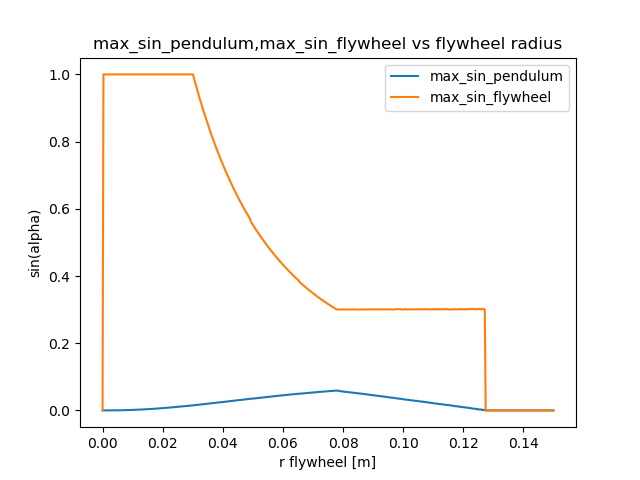
\includegraphics[width=10cm]{img/optimization/sin.png}
	\caption{Plot of the sinus of the maximum inclination in which the robot can keep his speed.}
	\label{fig:Sinus plot}
\end{figure}


\begin{figure}[ht]
	\centering
	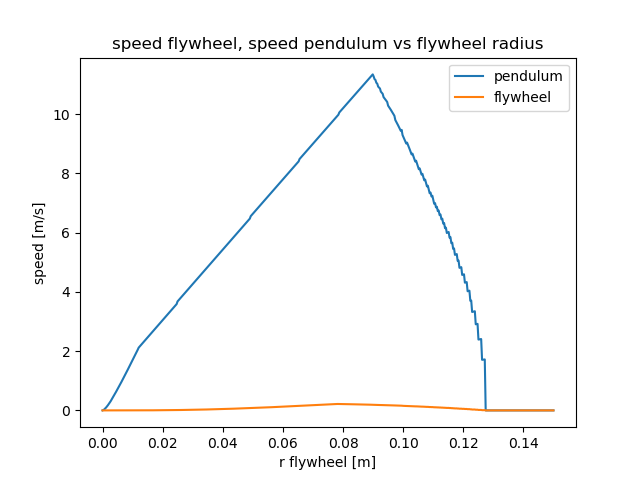
\includegraphics[width=10cm]{img/optimization/speed.png}
	\caption{Plot of the maximum speed that the robot can achieve.}
	\label{fig:Speed plot}
\end{figure}

\begin{figure}[ht]
	\centering
	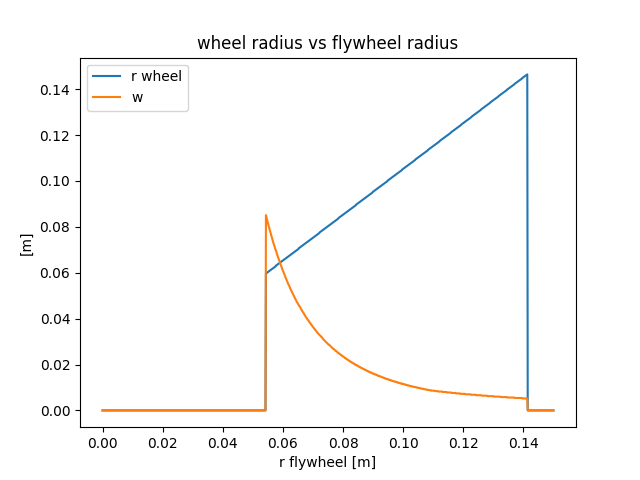
\includegraphics[width=10cm]{img/optimization/parameters.png}
	\caption{Plot of the parameters that maximize the cost function.}
	\label{fig:Parameters plot}
\end{figure}

\begin{figure}[ht]
	\centering
	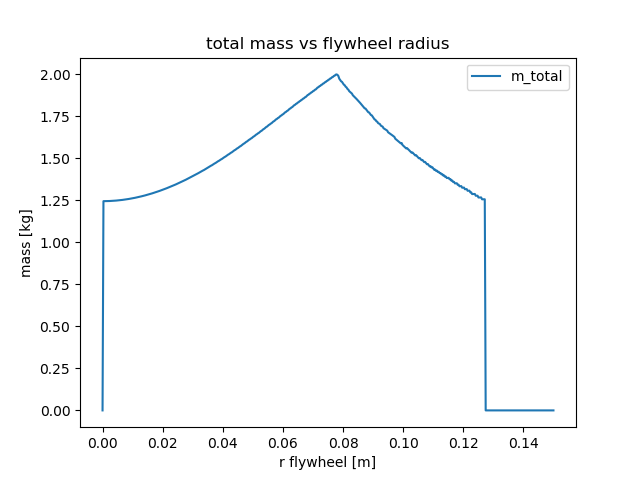
\includegraphics[width=10cm]{img/optimization/mass.png}
	\caption{Plot of the mass for each configuration.}
	\label{fig:Mass plot}
\end{figure}

